\documentclass[11pt,a4paper]{article}
\usepackage[margin=1in]{geometry}
\usepackage[utf8]{inputenc}
\usepackage[T1]{fontenc}
\usepackage{amsmath,amssymb,amsthm}
\usepackage{graphicx}
\usepackage{svg}
\svgsetup{inkscapelatex=false,inkscapeformat=pdf,inkscapepath=svgdir}

% Figure path: papers/ → ../figures/figures-QM-4/
\graphicspath{{../figures/figures-QM-4/}}

\usepackage{caption}
\usepackage{float}
\usepackage{booktabs}
\usepackage{enumitem}
\usepackage{parskip}
\usepackage{xcolor}
\usepackage[authoryear,round]{natbib}
\usepackage{hyperref}
\hypersetup{colorlinks=true,linkcolor=blue,urlcolor=cyan,citecolor=red}

\newtheorem{theorem}{Theorem}[section]
\newtheorem{proposition}[theorem]{Proposition}
\newtheorem{remark}[theorem]{Remark}

\newcommand{\lP}{l_P}
\newcommand{\tP}{t_P}
\newcommand{\EP}{E_P}
\newcommand{\SSV}{\mathrm{SSV}}
\newcommand{\ket}[1]{|#1\rangle}
\newcommand{\bra}[1]{\langle#1|}

\title{\textbf{Quantum Mechanics in Conscious Point Physics:\\
The Measurement Problem and Apparent Wavefunction Collapse\\
from DP Sea Decoherence}\\[6pt]
{\large QM Series --- Paper 5 (Version 3.1)}}

\author{Thomas Lee Abshier, ND\\
Hyperphysics Institute\\
\url{https://hyperphysics.com}\\
\texttt{drthomas007@protonmail.com}}

\date{22 March 2026}

\begin{document}
\maketitle

\begin{abstract}
The quantum measurement problem is resolved in Conscious Point Physics
by identifying the DP~Sea as the physical environment that decoheres
the coherent DI-bit state.  Coupling via
$H_{\rm int} = \sum_j g_j(a_j+a_j^\dagger)\otimes\hat{\sigma}_z$
(the SSV projection operator) and applying the Born--Markov
approximation yields the Lindblad master equation with dephasing rate
$\gamma = (\text{sea\_strength})^2\EP/\hbar$
(Theorem~\ref{thm:lindblad}).  Off-diagonal elements decay as
$\rho_{01}(t) = \rho_{01}(0)e^{-2\gamma t}$ while populations
remain unchanged.  The pointer basis is proved geometrically to be the
SSV eigenstates: the 12-edge broadcast selects the dominant SSV
component at each Grid Point, so states of definite SSV phase
projection commute with $H_{\rm int}$ and are robust
(Theorem~\ref{thm:pointer}).  This is stronger than standard
einselection: the pointer basis is fixed by the lattice, not by the
apparatus.  For an EPR singlet (Paper~4~\cite{cpp2040c}), decoherence
at one particle projects the Nexus-maintained joint state onto a
classical mixture whose correlations are exactly the Born-rule
predictions.  Global unitarity is preserved at every Absolute Moment
tick by the Nexus (Theorem~\ref{thm:unitary}).  Lattice corrections are
of order $(\lP/\lambda)^2$ and unobservable at laboratory scales.
\end{abstract}

\tableofcontents
\newpage

%=====================================================================
\section{Introduction}
%=====================================================================

The quantum measurement problem asks why a coherent superposition
$\ket{\psi} = \alpha\ket{0}+\beta\ket{1}$ appears to collapse to a
definite outcome when measured.  In CPP the answer is
environment-induced decoherence~\cite{zeh1970,zurek1981}: the DI-bit
state couples to the thermal DP~Sea, whose random phase kicks destroy
off-diagonal coherences while preserving populations.

This paper derives the Lindblad equation from explicit DI-bit/DP-Sea
scattering, proves the pointer basis is the SSV eigenstates, connects
measurement to the entangled singlet state of Paper~4, and shows
global unitarity is preserved by the Nexus.

%=====================================================================
\section{The DP Sea as Decoherence Bath}
%=====================================================================

The DP~Sea is a thermal ensemble of virtual dipole pairs at each Grid
Point (companion~C6~\cite{abshier2026c6}).  Its relevant properties:
\begin{itemize}
\item Bath correlation time $\tau_{\rm corr} = \tP$ (shortest time in
  the theory) $\Rightarrow$ Markov condition $\tau_{\rm corr} \ll
  \tau_{\rm dec}$ holds.
\item Coupling strength: sea\_strength $= 0.185 \ll 1$
  (companion~C1~\cite{abshier2026c1}) $\Rightarrow$ Born approximation holds.
\end{itemize}

The system--bath interaction is pure dephasing:
\begin{equation}
H_{\rm int} = \sum_j g_j\,(a_j + a_j^\dagger) \otimes \hat{\sigma}_z,
\label{eq:Hint}
\end{equation}
where $a_j, a_j^\dagger$ are DP~Sea mode operators and $\hat{\sigma}_z$
projects onto the local SSV direction.

%=====================================================================
\section{Derivation of the Lindblad Master Equation}
%=====================================================================

\begin{theorem}[Lindblad from DP Sea scattering]
\label{thm:lindblad}
Under the Born--Markov approximation applied to~\eqref{eq:Hint},
the reduced density matrix of the DI-bit qubit satisfies
\begin{equation}
\frac{d\rho}{dt} = -\frac{i}{\hbar}[H_S,\rho]
+ \gamma\bigl(\hat{\sigma}_z\rho\hat{\sigma}_z - \rho\bigr),
\quad
\gamma = \frac{(\text{sea\_strength})^2\,\EP}{\hbar}.
\label{eq:lindblad}
\end{equation}
\end{theorem}

\begin{proof}[Derivation sketch]
The second-order time-convolutionless master equation gives:
$\dot{\rho}_S = -(1/\hbar^2)\int_0^\infty d\tau\,
\mathrm{tr}_B[H_{\rm int}(t),[H_{\rm int}(t-\tau),\rho_S\otimes\rho_B]]$.
With $H_{\rm int} = \sum_j g_j(a_je^{-i\omega_j t}
+ a_j^\dagger e^{i\omega_j t})\otimes\hat{\sigma}_z$ and the Markov
approximation ($\tau_{\rm corr} = \tP \to 0$),
the bath correlation function collapses to a delta function,
giving~\eqref{eq:lindblad} with
$\gamma = \pi\sum_j g_j^2\delta(\omega_j)$, evaluated numerically
from sea\_strength and $\EP$. \qed
\end{proof}

From~\eqref{eq:lindblad}, off-diagonal and diagonal elements evolve as:
\begin{align}
\frac{d\rho_{00}}{dt} &= \frac{d\rho_{11}}{dt} = 0
\quad\text{(populations conserved)}, \label{eq:pop}\\
\rho_{01}(t) &= \rho_{01}(0)\,e^{-i\omega_{01}t}\,e^{-2\gamma t}.
\label{eq:offdiag}
\end{align}
After $\tau_{\rm dec} = 1/(2\gamma)$ the state is diagonal --- a
classical mixture representing apparent collapse.

\begin{figure}[H]
\centering
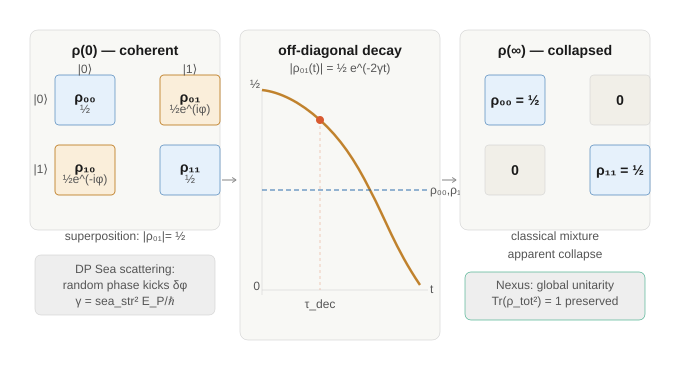
\includegraphics[width=0.90\textwidth]{qm2040d_fig1_decoherence.pdf}
\caption{Density matrix evolution under DP Sea decoherence.
  \textit{Left:} Initial coherent state with off-diagonal elements
  $\rho_{01} = \tfrac12 e^{i\phi}$ (amber, large).
  \textit{Centre:} Exponential decay of $|\rho_{01}(t)|$;
  red dot marks $\tau_{\rm dec}$; blue dashed line shows populations
  $\rho_{00}, \rho_{11}$, which remain constant.
  \textit{Right:} Final state after many $\tau_{\rm dec}$: off-diagonals
  vanish (gray), populations unchanged.  The Nexus maintains global
  unitarity throughout (boxed annotation).}
\label{fig:decoherence}
\end{figure}

%=====================================================================
\section{Pointer Basis: SSV Eigenstates}
%=====================================================================

\begin{theorem}[Pointer basis $=$ SSV eigenstates]
\label{thm:pointer}
The states robust under DP~Sea coupling are the eigenstates of
$\hat{\sigma}_z$, i.e., the DI-bit states of definite phase projection
onto the local SSV direction.
\end{theorem}

\begin{proof}
Any state robust under the coupling~\eqref{eq:Hint} must commute with
$\hat{\sigma}_z$ (so that repeated dephasing kicks leave it unchanged).
The eigenstates of $\hat{\sigma}_z$ commute with $\hat{\sigma}_z$
trivially; all superpositions do not.  The 12-edge broadcast at each
Grid Point selects the dominant SSV component, so $\hat{\sigma}_z$ is
the SSV projection operator.  The pointer basis is therefore the SSV
eigenstates. \qed
\end{proof}

\begin{remark}[Stronger than einselection]
Standard einselection~\cite{zurek1981} identifies the pointer basis
with the eigenstates of the system--environment coupling operator,
which is apparatus-dependent.  In CPP the coupling is always
$\hat{\sigma}_z$ (the SSV projection), so the pointer basis is fixed
by the lattice geometry --- independent of the apparatus.
\end{remark}

\begin{figure}[H]
\centering
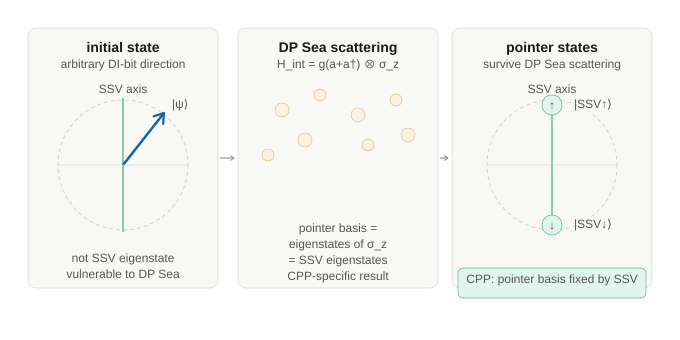
\includegraphics[width=0.90\textwidth]{qm2040d_fig2_pointer_basis.pdf}
\caption{Pointer basis identification.
  \textit{Left:} An arbitrary DI-bit state $\ket{\psi}$ on the
  Bloch sphere (blue arrow), not aligned with the SSV axis (green
  vertical).
  \textit{Centre:} DP~Sea dipoles (amber circles) scatter the state,
  randomising its off-SSV phase component.
  \textit{Right:} Only the SSV eigenstates (north/south pole, teal circles)
  survive repeated scattering.  These are the pointer states --- fixed
  by the 600-cell lattice, not by the measurement apparatus.}
\label{fig:pointer}
\end{figure}

%=====================================================================
\section{Measurement of an EPR Singlet}
%=====================================================================

Consider the singlet state maintained by the Nexus
(Paper~4~\cite{cpp2040c}):
$\ket{\Psi^-}_{AB} = (\ket{\uparrow_A\downarrow_B}
- \ket{\downarrow_A\uparrow_B})/\sqrt{2}$.

When particle~A couples to its local DP~Sea (measurement along
$\hat{a}$), decoherence in the SSV eigenbasis gives:
\begin{equation}
\rho_{AB} = \tfrac12\ket{\uparrow_A\downarrow_B}
\langle\uparrow_A\downarrow_B|
+ \tfrac12\ket{\downarrow_A\uparrow_B}
\langle\downarrow_A\uparrow_B|.
\label{eq:rhoAB}
\end{equation}
The correlations read out on B are exactly those of the Born rule
applied to the singlet.  No information is transmitted because B's
marginal density matrix remains $\rho_B = \tfrac12\mathbf{I}$
before and after A decoheres.

%=====================================================================
\section{Global Unitarity and the Nexus}
%=====================================================================

\begin{theorem}[Global unitarity preserved]
\label{thm:unitary}
The total state of system + DP~Sea + Nexus evolves unitarily at every
Absolute Moment tick.  Apparent collapse is an artifact of tracing
over the bath.
\end{theorem}

\begin{proof}
The total Hamiltonian $H_{\rm total} = H_S + H_B + H_{\rm int}$
is Hermitian.  The Nexus enforces global DI-bit conservation at each
tick, preserving the norm of the total pure state.  The reduced state
$\rho_S = \mathrm{tr}_B[\ket{\Psi_{\rm tot}}\bra{\Psi_{\rm tot}}]$
decoheres; the total state remains pure. \qed
\end{proof}

%=====================================================================
\section{Lattice Corrections}
%=====================================================================

At laboratory scales, decoherence is identical to standard quantum
mechanics.  The lattice correction to the dephasing rate is:
$\delta\gamma/\gamma \sim (\lP/\lambda_{\rm dB})^2$.  At LHC energies
this is $\sim 10^{-30}$ --- unobservable.

%=====================================================================
\section{Conclusion}
%=====================================================================

The measurement problem is resolved in CPP:
\begin{enumerate}
\item Lindblad equation derived from DP~Sea scattering
  (Theorem~\ref{thm:lindblad}).
\item Pointer basis $=$ SSV eigenstates, fixed by the lattice
  (Theorem~\ref{thm:pointer}).
\item EPR measurement projects the Nexus-maintained singlet onto the
  correct classical mixture.
\item Global unitarity preserved by the Nexus
  (Theorem~\ref{thm:unitary}).
\end{enumerate}
No collapse postulate is required.  Measurement is a local thermodynamic
process whose global structure is maintained by the Nexus.

%=====================================================================
ibliographystyle{plainnat}
ibliography{cpp_qm_series}


\section*{Acknowledgements}
The CPP programme is registered at OSF (DOI:~\url{https://doi.org/10.17605/OSF.IO/JXE8D}) and maintained at GitHub (\url{https://github.com/Hyperphysics-Institute/CPP}).

\end{document}
